\documentclass{article}
\usepackage[margin=1in]{geometry}
\usepackage{amsmath}
\usepackage{listings}
\usepackage{color}
\usepackage{graphicx}
\usepackage{blkarray}
\usepackage{multirow}

\definecolor{dkgreen}{rgb}{0,0.6,0}
\definecolor{gray}{rgb}{0.5,0.5,0.5}
\definecolor{mauve}{rgb}{0.58,0,0.82}

\lstset{frame=tb,
  language=Python,
  aboveskip=3mm,
  belowskip=3mm,
  showstringspaces=false,
  columns=flexible,
  basicstyle={\small\ttfamily},
  numbers=none,
  numberstyle=\tiny\color{gray},
  keywordstyle=\color{blue},
  commentstyle=\color{dkgreen},
  stringstyle=\color{mauve},
  breaklines=true,
  breakatwhitespace=true,
  tabsize=3
}

\begin{document}
\begin{titlepage}
	\setlength{\parindent}{0pt}
	\large

\vspace*{-2cm}

University of Waterloo \par
Econ 424 \par
2023-09-28 \par
\vspace{0.05cm}
Anonymized Usernmae: IJustWannaPass
\vspace{0.2cm}

{\huge Prediction Competition \# 3 \par}
\hrule

\vspace{1cm}
\textbf{Q1)} Due to some data manipulation I was able to get the following prediction accuracy of the training set:
\[ \text{Prediciton Accuracy} =  92.308\% \]
The normalized Confusion Matrix for this model on the training set is as follows (note we ran the 90-10 training test set 10 times):

\[\begin{tabular}{l|l|c|c|c}
\multicolumn{2}{c}{}&\multicolumn{2}{c}{Predicted Value}&\\
\cline{3-4}
\multicolumn{2}{c|}{}&0&1&\text{Total}\\
\cline{2-4}
\multirow{2}{*}{Actual Value}& 0 & $233786$ & $19778$ & $253564$\\
\cline{2-4}
& 1 & $18464$ & $227972$ & $246436$ \\
\cline{2-4}
\multicolumn{1}{c}{} & \multicolumn{1}{c}{Total} & \multicolumn{1}{c}{$252250$} & \multicolumn{    1}{c}{$227972$} & \multicolumn{1}{c}{$500000$}\\
\end{tabular}\] \\\\
\textbf{Q2)} The first graph showing how 1/k impacts the training and test error can be seen below:
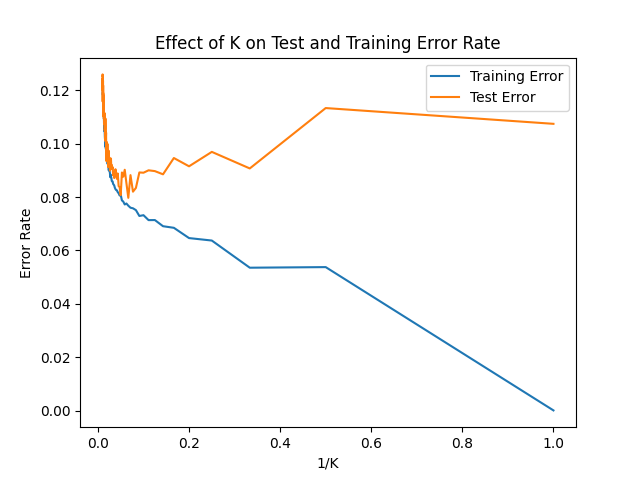
\includegraphics[width=\textwidth]{myplot.png}
As we can see the training error reduces as k/1 increases, however the test error first decreases and then increases as k/1 gets larger.
\newpage
\textbf{Q3)} The first graph showing the error rate and the classification curve is seen here: \\
\begin{center}
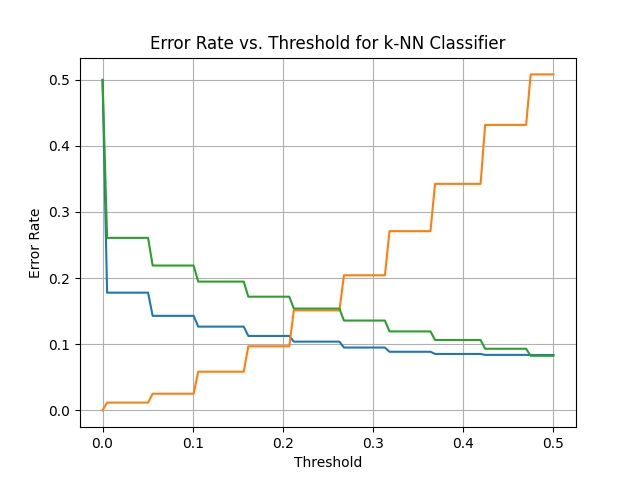
\includegraphics[width=0.8\textwidth]{thresh.png}
\end{center}
The second graph showing the ROC curve is seen below: \\
\begin{center}
\includegraphics[width=0.8\textwidth]{roccurve.png}
\end{center}
\newpage
\textbf{Q4)} To solve Q1 chatGPT was given the prompt: \\\\

\includegraphics[width=\textwidth]{q1prompt.png}
chatGPT provided the following response: \\\\
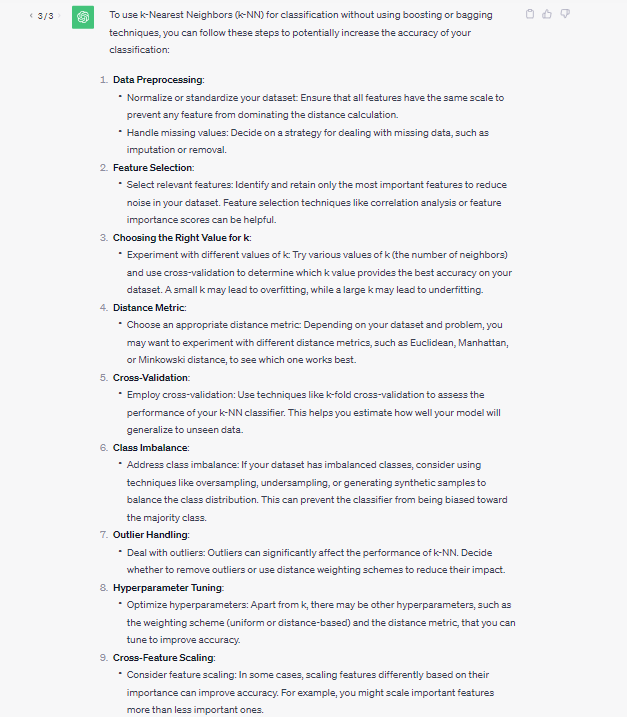
\includegraphics[width=\textwidth]{q1response.png}
To solve Q2 chatGPT was given the prompt: \\\\

\includegraphics[width=\textwidth]{q2prompt.png}
chatGPT provided the following response: \\\\
\begin{center}
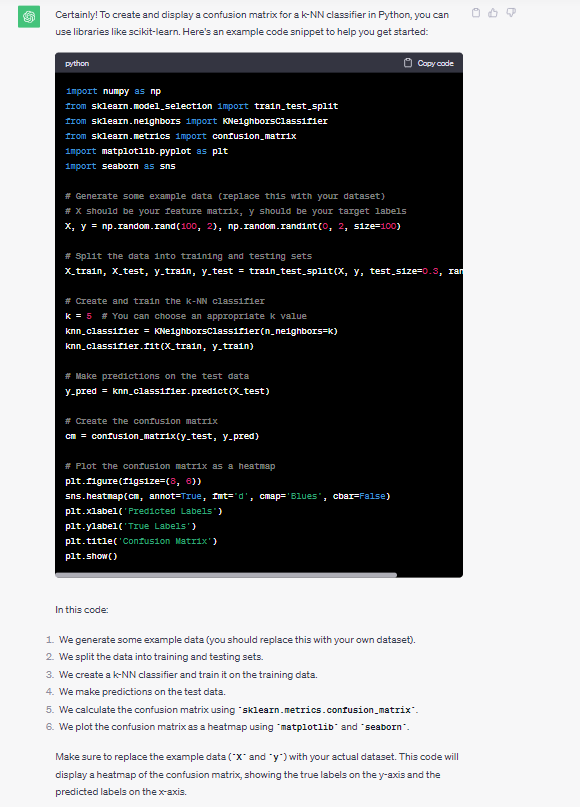
\includegraphics[width=0.8\textwidth]{q2response.png}
\end{center}
To solve Q3 chatGPT was given the prompt: \\\\

\includegraphics[width=\textwidth]{q3prompt.png}
chatGPT provided the following response: \\\\
\begin{center}
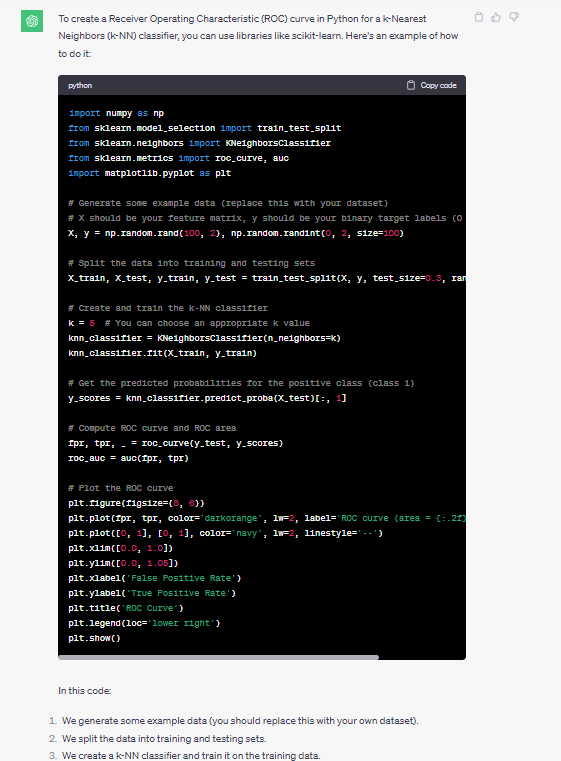
\includegraphics[width=0.8\textwidth]{q3response.png}
\end{center}

\end{titlepage}
\textbf{Code for Q1:}
\begin{lstlisting}
import matplotlib.pyplot as plt
import numpy as np
import pandas as pd

from sklearn.model_selection import train_test_split
from sklearn.neighbors import KNeighborsClassifier
from sklearn.metrics import ConfusionMatrixDisplay
# Read in the data
data = pd.read_csv("Econ_424_F2023_PC3_training_large.csv", low_memory=False)

# =============== DATA PREPROCESSING ===============

# Modify some of the columns that we wont be using
data.drop(columns=["city", "state", "make"], inplace=True)

# Some models are the same but use weird capitalization or ., this fixes that
data["model"] = data["model"].apply(lambda x: (str(x).lower()).split(".")[0])

# This function will keep a count of each model of car if its below or above 18400
#    ModelDict[model] = (#num cars above 18400, #num cars below 18400)
ModelDict = {}


def classify(price, dep):
    # Cluster cars without considering values after the .
    dep = dep.split(".")[0]

    above = 0
    below = 0
    if price >= 18400:
        above = 1
    else:
        below = 1

    if not dep in ModelDict:
        ModelDict[dep] = (above, below)
    else:
        ModelDict[dep] = (ModelDict[dep][0] + above, ModelDict[dep][1] + below)


data.apply(lambda x: classify(x['price'], x['model']), axis=1)

# This is the factor we use for assigning a numeric value to each car model, since from
#   looking at the data the model has a much greater fit with the price then the milage the
#   difference in model is equal to a value greater than the difference in mileage
diffFactor = 10 ** (int(np.log10(data["mileage"].max())) + 1)

# Since the number of large clusters is dynamic we start at 3 and keep growing
currLargeidx = 3
ModelWeights = {}

for key in ModelDict:
    if ModelDict[key][0] + ModelDict[key][1] < 30:
        # Only < 30 observations, cluster with similar small sample models

        if ModelDict[key][0] / (ModelDict[key][0] + ModelDict[key][1]) > 0.9:
            # Key belongs to above cluster (small)
            ModelWeights[key] = 2 * diffFactor
        elif ModelDict[key][1] / (ModelDict[key][0] + ModelDict[key][1]) > 0.9:
            # Key belongs to below cluster (small)
            ModelWeights[key] = 1 * diffFactor
        else:
            # Key belongs to either cluster (small)
            ModelWeights[key] = 0
    else:
        # Key belongs to its own cluster (enough observations)
        ModelWeights[key] = currLargeidx * diffFactor
        currLargeidx += 1

# Change the value of each model using the created dictionary
data["model"] = data["model"].map(lambda x: ModelWeights[x])
# Change the price to be 1 or 0 depending on price
data["price"] = data["price"].apply(lambda x: 1 if x < 18400 else 0)
# Change the year so that it the marginal year difference is worth more
data["year"] = data["year"].map(lambda x: x * (diffFactor / 10))

# =============== DATA TRAINING ===============


X_Train = [0] * 10
Y_Train = [0] * 10
X_Test = [0] * 10
Y_Test = [0] * 10

for i in range(0, 10):
    train, test = train_test_split(data, test_size=0.1)

    Y_Train[i] = train.iloc[:, 0]
    X_Train[i] = train.iloc[:, 1:]

    Y_Test[i] = test.iloc[:, 0]
    X_Test[i] = test.iloc[:, 1:]

neigh = KNeighborsClassifier(n_neighbors=19)

absError = 0
absCorrect = 0

predicted1Actual1 = 0
predicted1Actual0 = 0
predicted0Actual1 = 0
predicted0Actual0 = 0
for i in range(0, 10):
    neigh.fit(X_Train[i], Y_Train[i])
    predict = neigh.predict(X_Test[i])

    for idx in range(0, len(predict)):

        if predict[idx] == 0:
            if (Y_Test[i].iloc[idx] == 0):
                predicted0Actual0 += 1
            else:
                predicted0Actual1 += 1
        else:
            if (Y_Test[i].iloc[idx] == 0):
                predicted1Actual0 += 1
            else:
                predicted1Actual1 += 1

        # Calculations for Total Error
        if predict[idx] != Y_Test[i].iloc[idx]:
            absError += 1
        else:
            absCorrect += 1

print("Predicted:      0          1")
print("Actual [0]    " + str(round((predicted0Actual0 / (absCorrect + absError)) * 100, 2)) + "%    " + str(
    round((predicted1Actual0 / (absCorrect + absError)) * 100, 2)) + "%")
print("Actual [1]    " + str(round((predicted0Actual1 / (absCorrect + absError)) * 100, 2)) + "%    " + str(
    round((predicted1Actual1 / (absCorrect + absError)) * 100, 2)) + "%")



# =============== RUNNING THE PREDICTION ===============

Y_Train = data.iloc[:, 0]
X_Train = data.iloc[:, 1:]

neigh.fit(X_Train, Y_Train)

X_Test = pd.read_csv("Econ_424_F2023_PC3_test_without_response_variable.csv", low_memory=False)
X_Test.drop(columns=["city", "state", "make"], inplace=True)

def castModel(value ):
    if value == "mkxpremiere":
        return ModelWeights["mkxmkx"]
    if "s70" in value:
        return ModelWeights["s704dr"]
    if "lacrosse" in value:
        return ModelWeights["lacrossefwd"]
    if "routansel" in value:
        return ModelWeights["routan4dr"]
    if "caliber" in value:
        return 0
    if "eclipse" in value:
        return ModelWeights["eclipse2dr"]
    if "equinox" in value:
        return ModelWeights["equinoxawd"]
    if value in ModelWeights:
        return ModelWeights[value]
    else:
        # Assume it's in the pool of small sample observations
        return 0


X_Test["model"] = X_Test["model"].apply(lambda x: (str(x).lower()).split(".")[0])
X_Test["model"] = X_Test["model"].map(lambda x: castModel(x))
X_Test["year"] = X_Test["year"].map(lambda x: x * (diffFactor / 10))

estimates = neigh.predict(X_Test)

# Write the output
f = open('predictions.csv', 'w')
for estimate in estimates:
    f.writelines(str(estimate) + ",\n")
\end{lstlisting}
\newpage
\textbf{Code for Q2:}
\begin{lstlisting}
import matplotlib.pyplot as plt
import numpy as np
import pandas as pd

from sklearn.model_selection import train_test_split
from sklearn.neighbors import KNeighborsClassifier
# Read in the data
data = pd.read_csv("Econ_424_F2023_PC3_training_small.csv", low_memory=False)

# =============== DATA PREPROCESSING ===============

# Modify some of the columns that we wont be using
data.drop(columns=["city", "state", "make"], inplace=True)

# Some models are the same but use weird capitalization or ., this fixes that
data["model"] = data["model"].apply(lambda x: (str(x).lower()).split(".")[0])

# This function will keep a count of each model of car if its below or above 18400
#    ModelDict[model] = (#num cars above 18400, #num cars below 18400)
ModelDict = {}


def classify(price, dep):
    # Cluster cars without considering values after the .
    dep = dep.split(".")[0]

    above = 0
    below = 0
    if price >= 18400:
        above = 1
    else:
        below = 1

    if not dep in ModelDict:
        ModelDict[dep] = (above, below)
    else:
        ModelDict[dep] = (ModelDict[dep][0] + above, ModelDict[dep][1] + below)


data.apply(lambda x: classify(x['price'], x['model']), axis=1)

# This is the factor we use for assigning a numeric value to each car model, since from
#   looking at the data the model has a much greater fit with the price then the milage the
#   difference in model is equal to a value greater than the difference in mileage
diffFactor = 10 ** (int(np.log10(data["mileage"].max())) + 1)

# Since the number of large clusters is dynamic we start at 3 and keep growing
currLargeidx = 3
ModelWeights = {}

for key in ModelDict:
    if ModelDict[key][0] + ModelDict[key][1] < 30:
        # Only < 30 observations, cluster with similar small sample models

        if ModelDict[key][0] / (ModelDict[key][0] + ModelDict[key][1]) > 0.9:
            # Key belongs to above cluster (small)
            ModelWeights[key] = 2 * diffFactor
        elif ModelDict[key][1] / (ModelDict[key][0] + ModelDict[key][1]) > 0.9:
            # Key belongs to below cluster (small)
            ModelWeights[key] = 1 * diffFactor
        else:
            # Key belongs to either cluster (small)
            ModelWeights[key] = 0
    else:
        # Key belongs to its own cluster (enough observations)
        ModelWeights[key] = currLargeidx * diffFactor
        currLargeidx += 1

# Change the value of each model using the created dictionary
data["model"] = data["model"].map(lambda x: ModelWeights[x])
# Change the price to be 1 or 0 depending on price
data["price"] = data["price"].apply(lambda x: 1 if x < 18400 else 0)
# Change the year so that it the marginal year difference is worth more
data["year"] = data["year"].map(lambda x: x * (diffFactor / 10))

# =============== DATA TRAINING ===============

trainingResults = []
testResults = []
valsOverK = []
for k in range(1, 100, 1):
    neigh = KNeighborsClassifier(n_neighbors=k,n_jobs=-1)

    train, test = train_test_split(data, test_size=0.1)

    Y_Train = train.iloc[:, 0]
    X_Train = train.iloc[:, 1:]

    Y_Test = test.iloc[:, 0]
    X_Test = test.iloc[:, 1:]

    neigh.fit(X_Train, Y_Train)

    testPass = 0
    testError = 0

    trainingPass = 0
    trainingError = 0

    # Run tests of training data
    trainingPredict = neigh.predict(X_Train)
    for idx in range(0, len(trainingPredict)):
        if trainingPredict[idx] != Y_Train.iloc[idx]:
            trainingError += 1
        else:
            trainingPass += 1

    # Run tests of test data
    testPredict = neigh.predict(X_Test)
    for idx in range(0, len(testPredict)):
        if testPredict[idx] != Y_Test.iloc[idx]:
            testError += 1
        else:
            testPass += 1

    # Push the results onto an array to be printed later
    trainingResults.append(trainingError/(trainingPass+trainingError))
    testResults.append(testError/(testPass+testError))
    valsOverK.append(1 / k)

    print("====" + str(k) + "====")
    print("Training Results: " + str(trainingError/(trainingPass+trainingError)))
    print("Test Results: " + str(testError/(testPass+testError)))

plt.plot(valsOverK, trainingResults, label="Training Error")
plt.plot(valsOverK, testResults, label="Test Error")
plt.xlabel("1/K")
plt.ylabel("Error Rate")
plt.title("Effect of K on Test and Training Error Rate")
plt.legend()
plt.show()
\end{lstlisting}
\newpage
\textbf{Code for Q3:}
\begin{lstlisting}
import matplotlib.pyplot as plt
import numpy as np
import pandas as pd

from sklearn.model_selection import train_test_split
from sklearn.neighbors import KNeighborsClassifier
from sklearn.metrics import roc_curve, auc, accuracy_score, confusion_matrix
# Read in the data
data = pd.read_csv("Econ_424_F2023_PC3_training_small.csv", low_memory=False)

# =============== DATA PREPROCESSING ===============

# Modify some of the columns that we wont be using
data.drop(columns=["city", "state", "make"], inplace=True)

# Some models are the same but use weird capitalization or ., this fixes that
data["model"] = data["model"].apply(lambda x: (str(x).lower()).split(".")[0])

# This function will keep a count of each model of car if its below or above 18400
#    ModelDict[model] = (#num cars above 18400, #num cars below 18400)
ModelDict = {}


def classify(price, dep):
    # Cluster cars without considering values after the .
    dep = dep.split(".")[0]

    above = 0
    below = 0
    if price >= 18400:
        above = 1
    else:
        below = 1

    if not dep in ModelDict:
        ModelDict[dep] = (above, below)
    else:
        ModelDict[dep] = (ModelDict[dep][0] + above, ModelDict[dep][1] + below)


data.apply(lambda x: classify(x['price'], x['model']), axis=1)

# This is the factor we use for assigning a numeric value to each car model, since from
#   looking at the data the model has a much greater fit with the price then the milage the
#   difference in model is equal to a value greater than the difference in mileage
diffFactor = 10 ** (int(np.log10(data["mileage"].max())) + 1)

# Since the number of large clusters is dynamic we start at 3 and keep growing
currLargeidx = 3
ModelWeights = {}

for key in ModelDict:
    if ModelDict[key][0] + ModelDict[key][1] < 30:
        # Only < 30 observations, cluster with similar small sample models

        if ModelDict[key][0] / (ModelDict[key][0] + ModelDict[key][1]) > 0.9:
            # Key belongs to above cluster (small)
            ModelWeights[key] = 2 * diffFactor
        elif ModelDict[key][1] / (ModelDict[key][0] + ModelDict[key][1]) > 0.9:
            # Key belongs to below cluster (small)
            ModelWeights[key] = 1 * diffFactor
        else:
            # Key belongs to either cluster (small)
            ModelWeights[key] = 0
    else:
        # Key belongs to its own cluster (enough observations)
        ModelWeights[key] = currLargeidx * diffFactor
        currLargeidx += 1

# Change the value of each model using the created dictionary
data["model"] = data["model"].map(lambda x: ModelWeights[x])
# Change the price to be 1 or 0 depending on price
data["price"] = data["price"].apply(lambda x: 1 if x < 18400 else 0)
# Change the year so that it the marginal year difference is worth more
data["year"] = data["year"].map(lambda x: x * (diffFactor / 10))

# =============== DATA TRAINING ===============

trainingResults = []
testResults = []
valsOverK = []
neigh = KNeighborsClassifier(n_neighbors=19,n_jobs=-1)

train, test = train_test_split(data, test_size=0.1)

Y_Train = train.iloc[:, 0]
X_Train = train.iloc[:, 1:]

Y_Test = test.iloc[:, 0]
X_Test = test.iloc[:, 1:]

neigh.fit(X_Train, Y_Train)

y_scores = neigh.predict_proba(X_Test)[:,1]
# Compute ROC curve and ROC area
fpr, tpr, _ = roc_curve(Y_Test, y_scores)
roc_auc = auc(fpr, tpr)

# Plot the ROC curve
plt.figure(figsize=(8, 6))
plt.plot(fpr, tpr, color='darkorange', lw=2, label='ROC curve (area = {:.2f})'.format(roc_auc))
plt.plot([0, 1], [0, 1], color='navy', lw=2, linestyle='--')
plt.xlim([0.0, 1.0])
plt.ylim([0.0, 1.05])
plt.xlabel('False Positive Rate')
plt.ylabel('True Positive Rate')
plt.title('ROC Curve')
plt.legend(loc='lower right')
plt.show()

# Define a range of thresholds to test
thresholds = np.linspace(0.0, 0.5, 100)

# Initialize lists to store error rates
total_error = []
false_negative = []
false_positive = []

# Calculate error rates for different thresholds
for threshold in thresholds:
    y_pred = (neigh.predict_proba(X_Test)[:, 1] >= threshold).astype(int)
    error_rate = 1 - accuracy_score(Y_Test, y_pred)
    total_error.append(error_rate)

    tn, fp, fn, tp = confusion_matrix(Y_Test, y_pred).ravel()
    false_negative_rate = fn / (tp)
    false_postive_rate = fp / (fp + tn)

    false_negative.append(false_negative_rate)
    false_positive.append(false_postive_rate)

# Plot the relationship between threshold and error rate
plt.plot(thresholds, total_error)
plt.plot(thresholds, false_negative)
plt.plot(thresholds, false_positive)
plt.xlabel('Threshold')
plt.ylabel('Error Rate')
plt.title('Error Rate vs. Threshold for k-NN Classifier')
plt.grid(True)
plt.show()
\end{lstlisting}
\end{document}